\section{Основное содержание}

\subsection{Общий разбор темы}
Рассмотрим для начала определение аналогии с ресурса \cite{psychologsru}.

\begin{displayquote}
  ``Аналогия --- вид умозаключения; выявление свойств одного предмета на
  основании его сходства с другим. Аналогия --- один из общенаучных методов
  эмпирического и теоретического исследования. Аналогия не является строгим
  методом доказательства, однако применение аналогии часто приводит к более или
  менее правдоподобным предположениям о свойствах изучаемого объекта. Аналогия
  содействует переносу знаний по образцу, когда выполнение аналогичных заданий
  выступает условием формирования умения решать задачи данного типа. Аналогия
  способствует расширению познавательных возможностей учащихся, однако аналогию
  необходимо сочетать с более строгими формами доказательства''.
\end{displayquote}

На самом деле аналогия используется довольно часто при решении математических
задач. С её помощью можно сводить некоторое задачи из одной области математики
к другой, где существуют известные решения задачи как-либо похожих на исходную.
Это позволяет использовать те же "алгоритмы" или "шаблоны" которые
использовались раньше для решения подзадач, что существенно упрощает процесс
сопровождения задачи от ее осмысления до конкретного решения. В свою очередь
с точки зрения психологии встает вопрос как же 

Только в случае неудачи, которая может явиться следствием как недостаточного
запаса познаний, так и отсутствия вполне подходящих методов на современной
стадии развития науки, мы приступаем к самостоятельному поиску решения. Если мы
теперь проанализируем эти поиски, то увидим, что закулисная, сторона точного
мышления носит совсем другой характер, чем тот ряд теорем в готовом и
законченном виде, каждый член которого не колеблясь тянет последующие.

Точный разум, двигающей эту цепь теорем, повернут спиной по направлению своего
движения; он видит тот путь, который прошел, но не видит того, который ему
следует пройти. Один он шел бы действительно вперед; из посылки он вполне точно
выводил бы заключение, но он никогда бы не знал, куда идет, он не мог бы решить
ни одной наперед поставлен­ ной задачи. Решение какой бы то ни было задачи, не
подходящей прямо под общий случай, делающий решение чисто механическим, требует
по­ мощи гипотезирующего и колеблющегося разума. Мы делаем ряд попы­ ток, более
или менее удачных, при нахождении решения. Конечно, при выборе различных
путей для решения мы не предоставлены вполне игре воображения, Главным
двигателем здесь является аналогия. Если нам при­ ходит в голову та или иная
попытка, так именно потому, что она приносила успех в аналогичных случаях, Что
же касается степени аналогии данного случая со случаем известным, то эта
аналогия может быть весьма поверхностной.

\subsection{Дифференциальные уравнения}

Если нам дано какое-либо дифференциальное уравнение, то, отчаявшись подвести
это уравнение под уже известные типы, мы стараемся проинтегрировать его,
применяя различные методы, применявшиеся к интегрированию других аналогичных
дифференциальных уравнений. Но очевидно, что те аналогии, которые заставляют
блуждающую мысль остановиться на той или другой методе, часто не идут дальше
внешнего вида предложенного уравнения, Вполне естественно, если математику в
тот момент, когда он убедится, что уравнение:
\begin{equation}
  \left(a_0x+b_0\right)y^{(n)}
  + \left(a_1x+b_1\right)y^{(n-1)} 
  + \dots
  + \left(a_{n-1}x+b_{n-1}\right)y'y^{1} 
  + \left(a_nx+b_n\right)y
\end{equation}
не подходит ни под один из известных ему типов дифференциальных уравнений,
придет на мысль попытка интегрировать это уравнение подстановкой
$$y=e^{ax},$$
как линейное уравнение с постоянными коэффициентами. Конечно, такая мысль
придет только вследствие чисто внешней аналогии формы этих двух весьма
различных по своим свойствам уравнений.

У опытного математика не будет детального проведения этой по пытки, приводящей,
конечно, к неудаче, Такая мысль пробежит в один момент поле его сознания, так
как, при привычной ему быстроте в этой области соображения, неудача ему будет
почти очевидна. Но начинающий воспроизведет все выкладки.

Возьмем более сложный пример. Известно, что эйлеровское уравнение
\begin{equation}
  \frac{dx}{\sqrt{R(x)}}
  =
  \frac{dy}{\sqrt{R(y)}},
\end{equation}
где $R(x)$ полином 4-ой степени имеет алгебраический интеграл. Обобщение
эйлеровских исследований на случай, когда $R(x)$ полином какой угодно степени,
может иметь интерес и значение для науки. Бесспорно, что нe один исследователь,
до развития теории ультра-эллиптических интегралов, делал попытки обобщения,
при этом конечно он вполне доверялся по строенной им гипотезе о возможности
существования алгебраического интеграла у обобщенного эйлеровского уравнения.
Приступая затем к интегрированию такого уравнения, этот исследователь не
обладал другим оружием, кроме заключения по аналогии, и конечно первой мыслью
у негдолжна была бы явиться попытка применения к тому же уравнению те методов,
которые употреблял Эйлер для своего уравнения; эта попытка нe увенчалась бы
успехом, так как при производстве выкладок обнаружилось бы, что успех методы
Эйлера зависит от сокращения некоторых членов которые не сократятся в общем
случае, и поэтому в известном пункте цеп рассуждений обрывается. В этом примере
мы видим не только ошибочность предположения, относящегося к методе решения
предложенной проблемы, но и ошибочность сделанного предположения относительно
результата, который придает главным образом ценность исследуемой проблеме. 

Подобное описание механизма закулисной работы математической мысли согласно с
показаниями математиков. 

\begin{displayquote}
  ``В разговоре о роли воображения в научных трудах, --- говорит Либих, ---
  один великий французский математик выразил мнение, что большинство
  математических истин приобретены не дедукцией, а воображением''. 
\end{displayquote}

Далее рассмотрим некоторые другие типичные задачи, в которых используются
аналогии.

\subsection{Комплексные числа}

Изучая теорию функций комплексных переменных, мы часто интерпретируем
комплексное число геометрически. Имея комплексное число $z$ представленное в
виде:
\begin{equation}
  z = xi + y,
\end{equation}
можно представить его точкой на координатной плоскости, в Декартовой системе
координат, откладывая по одной из осей вещественную часть числа ($Re$), а по
другой мнимую ($Im$), с координатами $(x, y)$ как на рис.~\ref{fig:im}.
\begin{figure}[H]
  \centering
  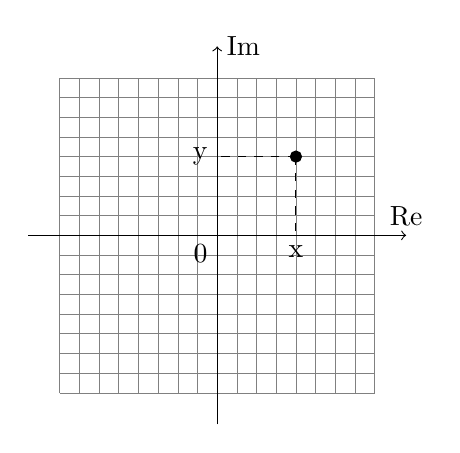
\begin{tikzpicture}
    \draw [help lines, step=0.25] (-2,-2) grid (2,2); 
    \draw [->] (-2.4,0) -- (2.4,0) node[above]{Re}; 
    \draw [->] (0,-2.4) -- (0,2.4) node[right]{Im}; 
    \filldraw (1, 1) circle (2pt);
    \draw [dashed] (1, 1) -- (1, 0) node[below]{x};
    \draw [dashed] (1, 1) -- (0, 1) node[left]{y};
    \draw (0,0) node[below left]{0};
  \end{tikzpicture}
  \caption{Представление комплексного числа на плоскости}\label{fig:im}
\end{figure}

Изменение $z$ мы представляем движением этой точки. Конечно, мы могли бы
изучать комплексные числа и чисто аналитически, не прибегая к геометрическому
образу.

\begin{theorem}\label{th:im}
  Модуль суммы меньше или равен сумме модулей
\end{theorem}

Теорему~\ref{th:im} мы можем доказать, не вводя геометрического представления
комплексного числа, хотя сложно не согласиться с тем, что эта теорема гораздо
легче доказывается геометрически.

\subsection{Абелев интеграл}

В настоящее время в анализе геометрический метод получил особенное
распространение, главным образом благодаря идеям Ф. Клейна. В двух отделах
чистой математики твердо установился геометрический характер мышления, в
теории дифференциальных уравнений, благодаря теории характеристик, и в теории
абелевых интегралов, благодаря исследованиям Клебша.

Абелев интеграл, т.е. интеграл от алгебраической функции можно представить в
форме 
\begin{equation}
  \int F(x,y)dx,
\end{equation}
где $F$ --- рациональная функция $(x,y)$, а $y$ определяется алгебраическим
уравнением
\begin{equation}
  f(x,y) = 0.
\end{equation}
Говорят, что Абелев интеграл $\int F(x,y)dx$ определяется алгебраической кривой
$f(x,y)=0$, воображая точку $(x,y)$, определяемую координатами $(x,y)$. Введя
этот геометрический язык, основную абелеву теорему можно сформулировать
следующим образом:

\begin{theorem}
Если пересечь кривую $f(x,y)=0$ некоторой деформирующейся кривой $\phi(x,y) =
0$, то сумма интегралов первого рода
\begin{equation}
  \sum\int\limits_{(x_0, y_0)}^{(x_i, y_i)} F(x,y)dx,
\end{equation}
относящихся к точкам пересечения этих кривых, сохраняет при деформировании
постоянное значение.
\end{theorem}

Не представляет труда освободить эту теорему от ее геометрической оболочки,
не представляет труда и все вытекающие из нее теоремы переложить с
геометрического языка на чисто алгебраической и можно продолжать мыслить,
двигая вперед теорию абелевых интегралов, отказавшись от всяких
геометрических образов. 

\subsection{Элементарные аналогии}

Аналогия так же полезна для объяснения некоторых задач на элементарном уровне,
например школьникам начальных классов. Примером такой простой аналогии может
быть сходство прямоугольника и параллелепипеда по соотношению граней.

\begin{displayquote}
  Прямоугольник схож с параллелепипедом.

  Каждая сторона прямоугольника параллельна и равна одной другой стороне и
  перпендикулярна остальным.

  Каждая грань прямоугольного параллелепипеда параллельна и равна одной другой
  грани и перпендикулярна остальным.
\end{displayquote}

Заметим так же, что не менее явная аналогия существует между площадью
прямоугольника и объемом параллелепипеда. Причем эта аналогия заключается не
только в самих формулах:
\begin{gather}
  S = a \times b
  \\
  V = a \times b \times c.
\end{gather}
Но и в структуре вывода этих формул.

\subsection{Четырехмерное пространство}

Если сознательная душевная жизнь не представляет всей полноты психической
жизни если сознание должно быть дополнено подсознанием, в котором психическими
явлениями управляют те же законы, которые мы усматриваем в области, озаренной
сознанием, то будет вполне естественно мыслить форм интуиции для расширенного
опыта бессознательной психики тоже шире Если сознанию доступна только
гиперплоскость, или только поверхность четырехмерного пространства, то в глубине
бессознательного может выступить интуиция четвертого измерения, не отвергающая
трехмерную геометрию, а дополняющая ее. 

Интуиция нам говорит, что то пространство, которое находится в нашем сознании,
имеет три измерения, но она ничего не может сказать о четвертом измерении,
которое оказывается под порогом сознания. 

Многие теоремы четырехмерного пространства могут быть построены
непосредственно, как аналогии соответствующих теорем трехмерного
пространства. Примером ряда поиятий-аналогонов может служит ряд простейших
образов: 
\begin{enumerate}
  \item в пространстве;
  \item одного измерения --- две точки;
  \item двух --- три прямые --- треугольник;
  \item трех --- четыре плоскости --- тетраэдр;
\end{enumerate}
Следуя правилу, по которому переходили от одного аналогона к следующему, можем
четвертым членом упомянутого ряда поставить в пространстве 4х измерений
четырехмерное тело, образованное пятью гиперплоскостями --- пентаэдроид.

Изучение пентаэдроида производится проектированием его в гиперплоскость,
которую представляет все наше трехмерное пространство.

Чтобы получить проекцию треугольника на прямую, надо взять три точки на прямой
и отрезки ими образуемые, тетраэдра на плоскости --- четыре точки на плоскости
и треугольники, ими образуемые. Отсюда следует, что проекция пентаэдра
получится, если взять пять точек в пространстве (гиперплоскости) и пять
тетраэдров, ими образуемых. 

Можно, следуя правилу аналогонов, создать и механику четырех мерного
пространства. 

В механике четырехмерного пространства приходится, следуя аналогии трехмерной
механики, рассматривать при движении точки ее четыре координаты: $x$, $y$, $z$,
$u$, как функции времени $\tau$. 

Движение будет происходить в гиперплоскости, т.е. в нашем трех мерном
пространстве, если $x$, $y$, $z$, и для всякого $\tau$ связаны линейным 
соотношением: 
\begin{equation}
  Ax + By + Cz + Du + E = 0,
\end{equation}
представляющими уравнение гиперплоскости.

Мы получим уравнение движения на некоторой гиперповерхности, если свяжем ($x$,
$y$, $z$, $u$) общим уравнением: 
\begin{equation}
  \Omega(x, y, z, u) = 0
  \label{eq:move}
\end{equation}
Можно сделать такое предположение: наше пространство не гиперплоскость, а
некоторая, отличная от нее гиперповерхность; для четырехмерного пространства
(а следовательно и для гиперплоскостей, в нем заключающихся) объемлющего эту
гиперповерхность имеет место неевклидова геометрия. Источником ошибочного
взгляда на наше пространство, как пространство евклидово, служит то, что мы
некоторые кривые, мало отличающиеся от прямых, принимаем за прямые, приписывая
последним те свойства, которые на самом деле присущи первым. 

Воздерживаясь от возражений на эти взгляды, укажем, в каком направлении должно
идти дальнейшее их обобщение. Для этого следует только уравнение
(\ref{eq:move}) заменить более общим 
\begin{equation}
  \Omega(x, y, z, u, \tau) = 0
\end{equation}
т.е. принять эту гиперповерхность деформирующейся в течение времени.
 
В этого рода пространстве и строится механика Минковского. Фи зические явления
происходят в четырехмерном пространстве ($x$, $y$, $z$, $u$). Но, что
представляет собой координата $u$? 

Этой координатой является время $t$., но только иное, чем упомяну­
тое выше $\tau$. 

В механике Минковского приходится различать абсолютное время $t$ от
собственного $\tau$. 

В этих воззрениях мы имеем не одно пространство, а особое сочетание
пространство-время, находящееся в таком же отношении к геометрическому
пространству и абсолютному времени, в каком у эмпириков-метагеометров
неевклидово пространство находится в отношении к евклидову. 

Возражения, упомянутые нами, остаются и здесь еще в большей силе. 

Но воззрения Минковского имеют еще свой специальный недостаток: это
чрезвычайная сложность и искусственность. 

Если в них видеть нечто большее, чем одну геометрическую интерпретацию, то надо
сознаться, что фигурирование четвертого измерения
времени, наряду с однородными другими тремя измерениями, совершенно
отличными от этого четвертого, уже достаточно для того, чтобы признать
весь этот сложный аппарат хотя и гениально задуманным, но совершенно
невероятным. 






